\clearpage
\section{BB84 with Discrete Variables}

\begin{tcolorbox}	
\begin{tabular}{p{2.75cm} p{0.2cm} p{10.5cm}} 	
\textbf{Students Name}  &:& Mariana Ramos and Kevin Filipe\\
\textbf{Starting Date} &:& November 7, 2017\\
\textbf{Goal}          &:& BB84 implementation with discrete variables.
\end{tabular}
\end{tcolorbox}

BB84 is a key distribution protocol which involves three parties, Alice, Bob and Eve. Alice and Bob exchange information between each other by using a quantum channel and a classical channel. The main goal is continuously build keys only known by Alice and Bob, and guarantee that eavesdropper, Eve, does not gain any information about the keys.



\subsection{Theoretical Description}

BB84 protocol was created by Charles Bennett and Gilles Brassard in 1984. This was the first created Quantum Key Distribution (QKD) protocol. A basic model is depicted in figure \ref{fig:qkd model}. It involves two parties sharing keys through a quantum channel to decipher the classical channel data with an eavesdropper, Eve, between them.


\begin{figure}[H]
	\centering
	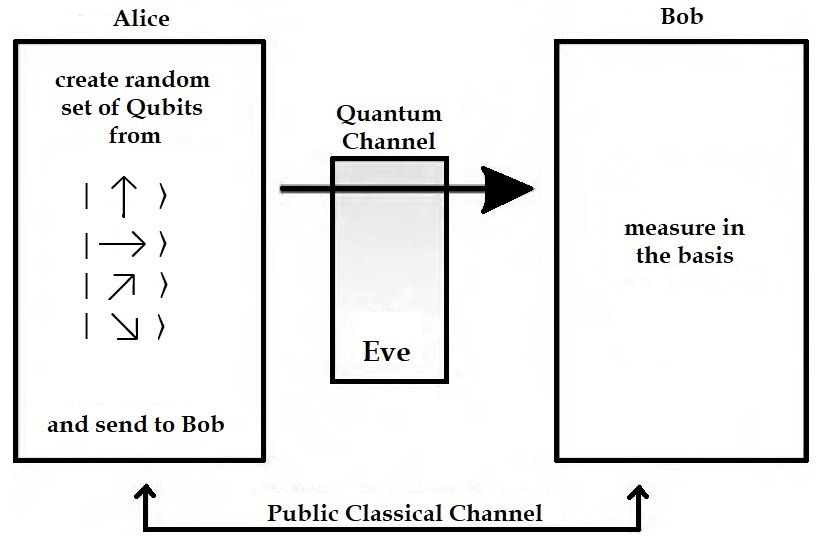
\includegraphics[width=1.0\textwidth,height=7cm]{./sdf/bb84_with_discrete_variables/figures/QKD_Model.png}
	\caption{Basic QKD Model.}\label{fig:qkd model}
\end{figure}

BB84 protocol encodes bits into photon state polarization. This either can have an angle of 0 or 45 degrees, to represent bit 0, or an angle of 90 or 135 degrees, to represent bit 1, in rectilinear or diagonal basis, respectively. Figure \ref{fig:bb84_encoding} shows this bit encoding and basis.

\begin{figure}[H]
	\centering
	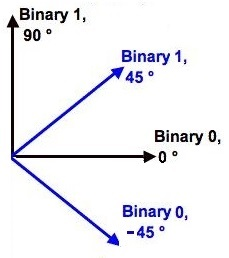
\includegraphics[width=0.5\textwidth,height=7cm]{./sdf/bb84_with_discrete_variables/figures/basis.png}
	\caption{Bit Encoding and polarization basis.}\label{fig:bb84_encoding}
\end{figure}
The BB82 protocol is divided in different phases. For the first phase, by using the quantum communication channel,
\begin{enumerate}
	\item Alice chooses a random bit string and polarization, for each bit.
	\item For each bit, a photon is transmitted, with an associated polarization, to Bob.
	\item Bob receives, measure photon polarization by using a random basis.
	\item If Bob chooses a matched polarization basis compared to the one encoded in the photon, then he can correctly deduce the right bit, otherwise deduced bit is randomly read.
\end{enumerate}

The second phase, uses the classical communication channel:
\begin{enumerate}
	\item Bob notifies Alice about what basis he used to deduce each bit.
	\item Alice announces, to Bob, if the deduced basis is correct for each photon, and so, discards the bits measured with different one.
	\item If no errors occurred the secret key should be the same for Bob and Alice.
\end{enumerate}

This two phases are depicted in figure \ref{fig:bb84_share}.

\begin{figure}[H]
	\centering
	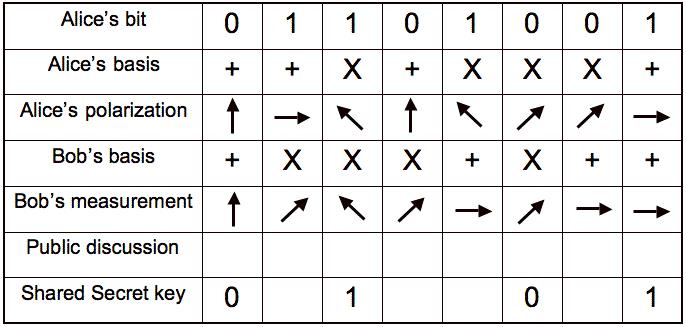
\includegraphics[width=0.5\textwidth,height=4cm]{./sdf/bb84_with_discrete_variables/figures/siftedKey.png}
	\caption{Bit Encoding and polarization basis.}\label{fig:bb84_share}
\end{figure}

In the presence of Eve, error will be introduced, because for Eve to determine the key, she will have to measure the photons sent between Alice and send them to Bob. By doing so, errors will be introduced since its impossible to replicate a particle with an unknown state. Eve will try to guess and these guesses will increase the QBER.
--/--/--/--/





\begin{table}[H]
\centering
\begin{tabular}{c|c}
\textbf{\textit{Basis}}         &  \\ \hline
 0 & $+$ \\
 1 & $\times$ \\
\end{tabular}
\end{table}


\begin{table}[H]
\centering
\begin{tabular}{c|c}
            & Basis "+" \\ \hline
 0 & $\to (0^{\circ})$ \\
 1 & $\uparrow (90^{\circ})$ \\
\end{tabular}
\end{table}


\begin{table}[H]
\centering
\begin{tabular}{c|c}
      & Basis "$\times$" \\ \hline
 0 & $\searrow (-45^{\circ})$ \\
 1 & $\nearrow (45^{\circ})$ \\
\end{tabular}
\end{table}


\begin{enumerate}
  \item Alice randomly generate a bit sequence with length $ks$ being, in this case, $k=2$ and $s=4$ as it was defined at the beginning.
      Therefore, she must define two sets randomly: $S_{A1}$ which contains the basis values; and $S_{A2}$, which contains the key values.

      In that case, lets assume she gets the following sets $S_{A1}$ and $S_{A2}$:
      $$S_{A1} = \{0,1,1,0,0,1,0,1 \},$$
      $$S_{A2} = \{1,1,0,0,0,1,0,0 \}.$$

  \item Next, Alice sends to Bob throughout a quantum channel $ks$ photons encrypted using the basis defined in $S_{A1}$ and according to the keys defined in $S_{A2}$.

      In the current example, Alice sends the photons, throughout a quantum channel, according to the following,

      $$S_{AB} = \{\uparrow, \nearrow, \searrow, \to, \to, \nearrow, \to, \searrow \}.$$
       $$S_{AB} = \{90^{\circ}, 45^{\circ}, -45^{\circ}, 0^{\circ}, 0^{\circ}, 45^{\circ}, 0^{\circ}, -45^{\circ} \}.$$

  \item Bob also randomly generates $ks$ bits, which are going to define his measurement basis, $S_{B1}$. He will measure the photons sent by Alice. Lets assume:

  $$S_{B1} = \{0,1,0,1,0,1,1,1 \}.$$

    When Bob receives photons from Alice, he measures them using the basis defined in $S_{B1}$.
  In the current example, $S_{B1}$ corresponds to the following set:
  $$\{ +,\times,+,\times,+,\times, \times, \times \}.$$
  Bob will get $ks$ results:
  $$S_{B1'} = \{1,1,0,1,0,1,1,0 \}.$$

  \item Bob will send a \textit{Hash Function} result HASH1 to Alice. This value will do Bob's commitment with the measurements done. In this case, this \textit{Hash Function} is calculated from \textit{SHA-256} algorithm for each pair (Basis from $S_{B1}$ and measured value from $S_{B1'}$), i.e Bob sends to Alice $sk$ pairs as his commitment. In this case, Bob sends eight pairs encoded using a \textit{Hash Function} which is also send to Alice. From that moment on Bob cannot change his commitment neither the basis which he uses to measure the photons sent by Alice.

  \item Once Alice has received the confirmation of measurement from Bob, she sends throughout a classical channel the basis which she has used to codify the photons, which in this case we assumed $S_{A1} = \{0,1,1,0,0,1,0,1\}$.

  \item In order to know which photons were measured correctly, Bob does the operation $S_{B2}=S_{B1} \oplus S_{A1}$.
      In the current example the operation will be:

  \begin{table}[H]
    \centering
    \begin{tabular}{c|c c c c c c c c}
     $S_{B1}$ & 0 & 1 & 0 & 1 & 0 & 1 & 1 & 1 \\
     $S_{A1}$ & 0 & 1 & 1 & 0 & 0 & 1 & 0 & 1 \\ \hline
     $\oplus$ & 1 & 1 & 0 & 0 & 1 & 1 & 0 & 1
    \end{tabular}
    \end{table}

      In this way, Bob gets $$S_{B2} = \{1,1,0,0,1,1,0,1 \}.$$ When Bob uses the right basis he gets the values correctly, when he uses the wrong basis he just guess the value. The values ``$1$'' correspond to the values he measured correctly and ``$0$'' to the values he just guessed.

       Next, Bob sends to Alice, through a classical channel, information about the minimum number between ``ones'' and ``zeros'', i.e $$n=min(\#0,\#1)=3,$$ where $\#0$ represents the number of zeros in $S_{B2}$ and $\#1$ the number of ones in $S_{B2}$. At this time, Alice must be able to know if Bob is being honest or not. Therefore, she will open Bob's commitment from \textit{step 4} and she verify if the number n sent by Bob is according with the commitment values sent by him. In other words, she opens a number of pairs committed by Bob which is known from the beginning.

  \item If $n<s$, being \textit{s} the message's size, Alice and Bob will repeat the steps from $1$ to $7$. In this case, $n=3$ which is smaller than $s=4$. Therefore, Alice and Bob repeat the steps from 1 to 7 in order to enlarge Bob's sets $S_{B1}$ and $S_{B2}$ as well as Alice's sets $S_{A1}$ and $S_{A2}$.

  \item Lets assume :

   $$S_{B1}= \{1,1,0,0,0,1,0,0,1,0,0,0,0,0,1,1 \}.$$

    At Alice's side the new sets $S_{A1}$, which contains the basis values, and $S_{A2}$, which contains the key values, will be the following:

    $$S_{A1}=\{0,1,1,0,0,1,0,1,1,1,0,0,1,1,1,0 \},$$ $$S_{A2}=\{1,1,0,0,0,1,0,0,1,0,1,0,0,0,1,1 \}.$$

    Finally, for $S_{B2}=S_{B1} \oplus S_{A1}$ Bob gets the following sequence:

    $$S_{B2}= \{1,1,0,0,1,1,0,1,0,1,0,0,1,1,0,1 \}.$$

    Note that the sets were enlarge in the second iteration.

  \item At this time, Bob sends again to Alice, through a classical channel, the minimum number between  ``ones'' and ``zeros'',  $n=min(\#0,\#1)$. In this case, $n$ is equal to $7$ which is the number of zeros.

  \item Alice checks if $n>s$ and acknowledge to Bob that she already knows that $n>s$. In this case, $n=7$ and $s=4$ being $n>s$ a valid condition.

  \item Next, Bob defines two new sub-sets, $I_{0}$ and $I_{1}$. $I_{0}$ is a set of values with photons array positions which Bob just guessed the measurement since he did not measure them with the same basis as Alice, $I_{1}$ is a set of values with photons array positions which Bob measured correctly since he used the same basis as Alice used to encoded them.

  In this example, Bob defines two sub-sets with size $s=4$:
  $$I_{0}=\{3,4,7,11 \},$$
  and $$I_{1}= \{2,5,6,13 \},$$ where $I_{0}$ is the sequence of positions in which Bob was wrong about basis measurement and $I_{1}$ is the sequence of positions in which Bob was right about basis measurement. Bob sends to Alice the set $S_{b}$

  Thus, if Bob wants to know $m_{0}$ he must send to Alice throughout a classical channel the set $S_{0}=\{I_{1},I_{0} \}$, otherwise if he wants to know $m_{1}$ he must send to Alice throughout a classical channel the set $S_{1}=\{I_{0},I_{1} \}$.


  \item With both the received set $S_{b}$ and the hash function value HASH1, Alice must be able to prove that Bob has being honest.

  \item Lets assume Bob sent $S_{0}=\{I_{1},I_{0} \}$.
   Alice defines two encryption keys $K_{0}$ and $K_{1}$ using the values in positions defined by Bob in the set sent by him. In this example, lets assume: $$K_{0}=\{1,0,1,0\}$$ $$K_{1}=\{0,0,0,1\}.$$

   Alice does the following operations:
   $$m = \{m_{0}\oplus K_{0}, m_{1} \oplus K_{1} \}.$$

   \begin{table}[H]
    \centering
    \begin{tabular}{c|c c c c c c c c}
     $m_{0}$ & 0 & 0 & 1 & 1 \\
     $K_{0}$ & 1 & 0 & 1 & 0 \\ \hline
     $\oplus$ & 1 & 0 & 0 & 1
    \end{tabular}
    \end{table}

   \begin{table}[H]
    \centering
    \begin{tabular}{c|c c c c c c c c}
     $m_{1}$ & 0 & 0 & 0 & 1 \\
     $K_{1}$ & 0 & 0 & 0 & 1 \\ \hline
     $\oplus$ & 0 & 0 & 0 & 0
    \end{tabular}
    \end{table}

    Adding the two results, $m$ will be: $$m=\{1,0,0,1,0,0,0,0\}.$$

   After that, Alice sends to Bob the encrypted message $m$ through a classical channel.

  \item When Bob receives the message $m$, in the same way as Alice, Bob uses $S_{B1\prime}$ values of positions given by $I_{1}$ and $I_{0}$ and does the decrypted operation. In this case, he does following operation:

      \begin{table}[H]
        \centering
        \begin{tabular}{c|c c c c c c c c}
         $m$ & 1 & 0 & 0 & 1 & 0 & 0 & 0 & 0 \\
             & 1 & 0 & 1 & 0 & 0 & 1 & 1 & 0 \\ \hline
         $\oplus$ & 0 & 0 & 1 & 1 & 0 & 1 & 1 & 0 \\
        \end{tabular}
        \end{table}

      The first four bits corresponds to message 1 and he received $\{0,0,1,1\}$, which is the right message $m_{0}$ and $\{0,1,1,0\}$ which is a wrong message for $m_{1}$.


\end{enumerate}

\subsection{Simulation Setup}



\begin{figure}[H]
	\centering
	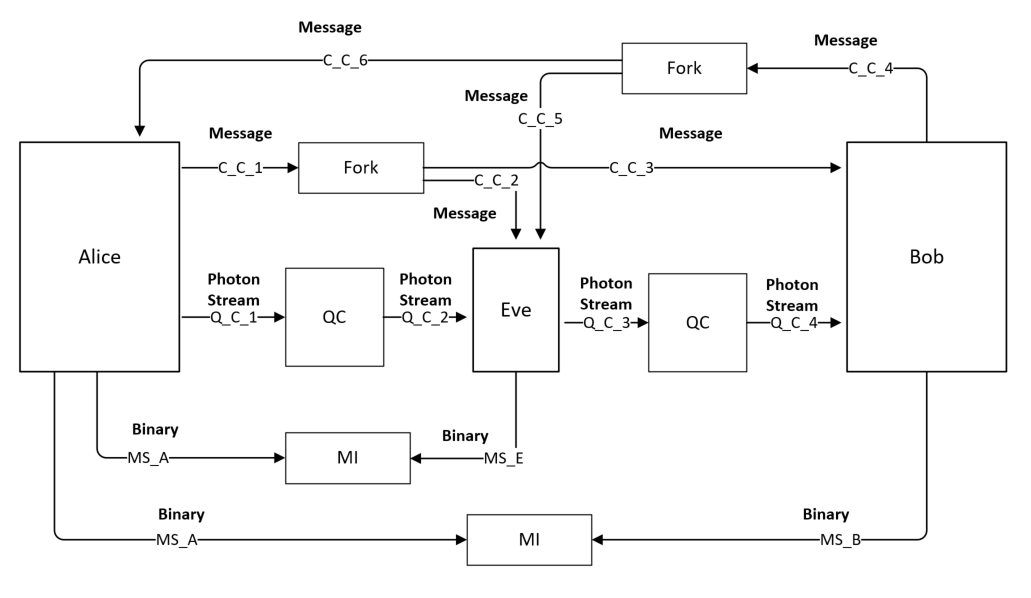
\includegraphics[width=1.0\textwidth, height=9cm]{./sdf/bb84_with_discrete_variables/figures/toplevel_simulation.png}
	\caption{Simulation diagram at a top level}\label{toplevelsimulation}
\end{figure}

Figure \ref{toplevelsimulation} presents the top level diagram of our simulation. The setup contains three parties, Alice, Eve and Bob where the communication between them is done throughout two classical and one quantum channel. In the middle of the classical channel there is a Fork's diagram which has one input and two outputs. In the case of the classical channel \textbf{C\_C\_4} which has the information sent by Bob, the fork's block enables Alice and Eve have access to it. In the quantum communication, the information sent by Alice can be intercepted by Eve and changed by her, or can follow directly to Bob as we can see later in figure \ref{evesimulation}. Furthermore, for mutual information calculation there must be two blocks \textbf{MI}, one to calculate the mutual information between Alice and Eve, and other to calculate the mutual information between Alice and Bob.

\begin{figure}[h]
	\centering
	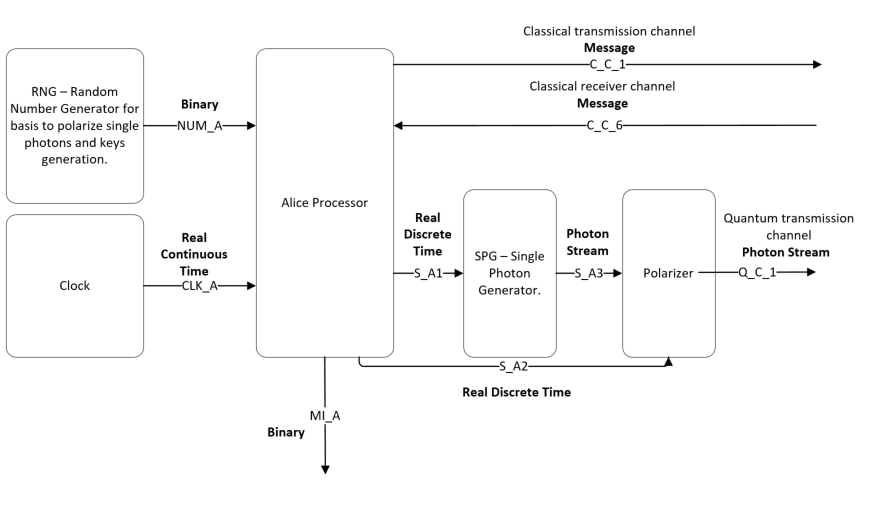
\includegraphics[width=1.0\textwidth, height=9cm]{./sdf/bb84_with_discrete_variables/figures/alice_simulation.png}
	\caption{Simulation diagram at Alice's side}\label{alicesimulation}
\end{figure}

\begin{figure}[h]
	\centering
	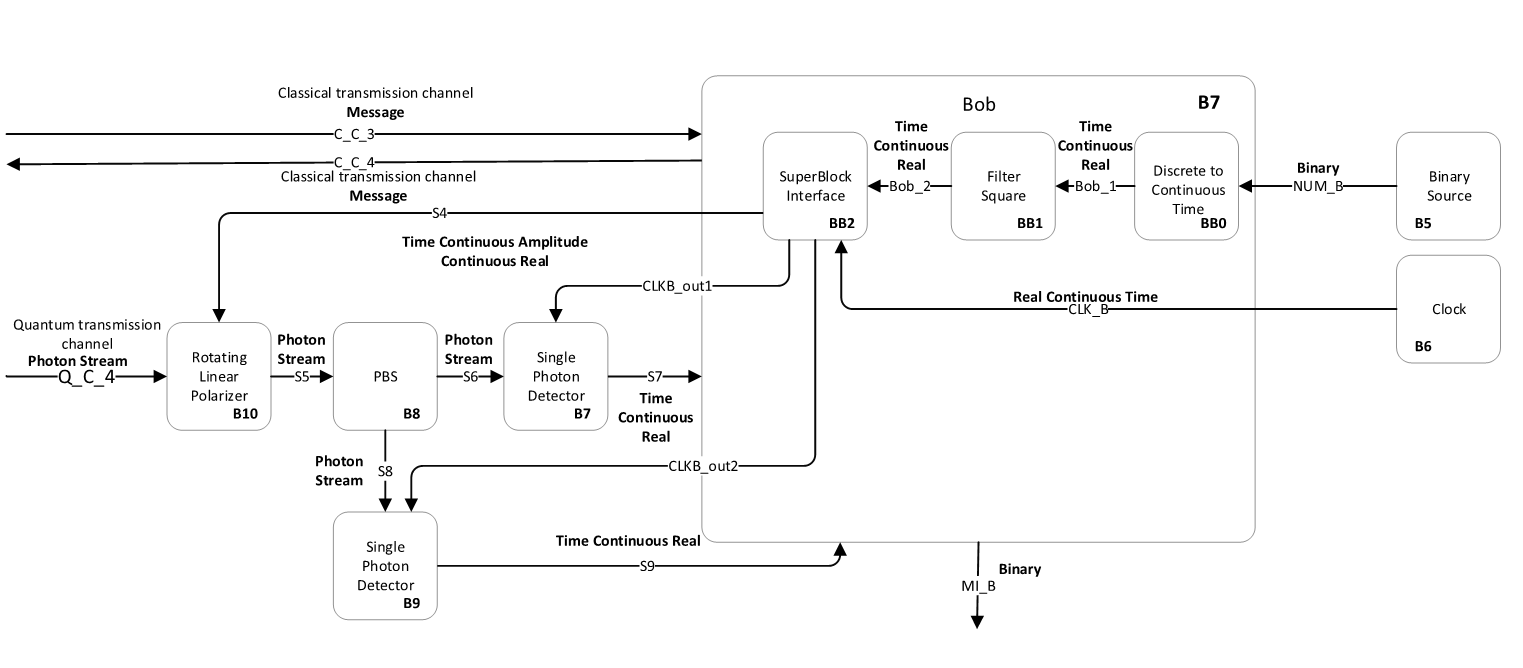
\includegraphics[width=1.0\textwidth, height=9cm]{./sdf/bb84_with_discrete_variables/figures/bob_simulation.png}
	\caption{Simulation diagram at Bob's side}\label{bobsimulation}
\end{figure}

    In figure \ref{alicesimulation} one can observe a block diagram of the simulation at Alice's side. As it is shown in the figure, Alice must have one block for random number generation which is responsible for basis generation to polarize the photons, and for key random generation in order to have a random state to encode each photon. Furthermore, she has a Processor block for all logical operations: array analysis, random number generation requests, and others. This block also receives the information from Bob after it has passed through a fork's block. In addition, it is responsible for set the initial length $l$ of the first array of photons which will send to Bob. This block also must be responsible for send classical information to Bob. Finally, Processor block will also send a real continuous time signal to single photon generator, in order to generate photons according to this signal, and finally this block also sends to the polarizer a real discrete signal in order to inform the polarizer which basis it should use. Therefore, she has two more blocks for quantum tasks: the single photon generator and the polarizer block which is responsible to encode the photons generated from the previous block and send them throughout a quantum channel from Alice to Bob.

    Finally, Alice's processor has an output to Mutual Information top level block, $Ms_{A}$.

     In figure \ref{bobsimulation} one can observe a block diagram of the simulation at Bob's side. From this side, Bob has one block for Random Number Generation which is responsible for randomly generate basis values which Bob will use to measure the photons sent by Alice throughout the quantum channel. Like Alice, Bob has a Processor block responsible for all logical tasks, analysing functions, requests for random number generator block, etc. Additionally, it receives information from Alice throughout a classical channel after passed through a fork's block and a quantum channel. However, Bob only sends information to Alice throughout a classical channel. Furthermore, Bob has one more block for single photon detection which receives from processor block a real discrete time signal, in order to obtain the basis it should use to measure the photons.

    Finally, Bob's processor has an output to Mutual Information top level block, $Ms_{B}$.



\begin{figure}[h]
	\centering
	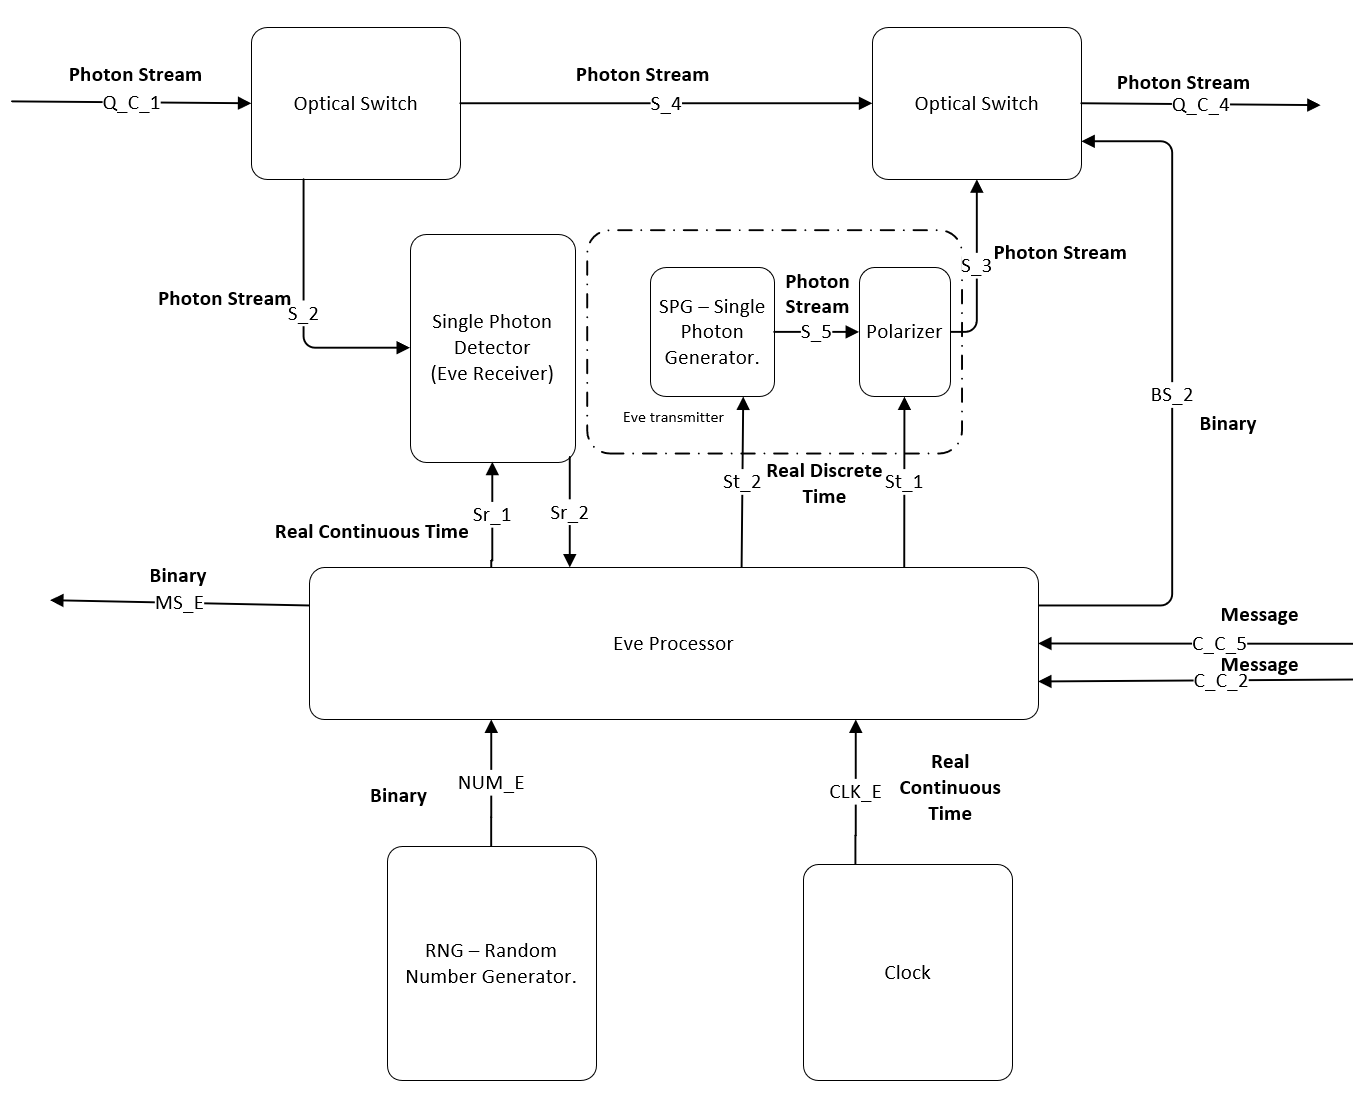
\includegraphics[width=1.1\textwidth, height=14cm]{./sdf/bb84_with_discrete_variables/figures/eve_simulation.png}
	\caption{Simulation diagram at Eve's side}\label{evesimulation}
\end{figure}

Figure \ref{evesimulation} presents the Eve's side diagram. Eve's processor has two receiver classical signals, one from Alice (\textbf{C\_C\_2}) and other from Bob (\textbf{C\_C\_5}). About quantum channel, Eve received a quantum message from Alice through the channel \textbf{Q\_C\_1} and depends on her decision the photon can follows directly to Bob or the photon's state can be changed by her. In this case, the photon is received by a block similar to Bob's diagram \ref{bobsimulation} and this block sends a message to Eve's processor in order to reveal the measurement result. After that, Eve's processor sends a message to Alice's diagram similar to figure \ref{alicesimulation} and this block is responsible for encode the photon in a new state. Now, the changed photon is sent to Bob.

In addition, Eve's diagram has one more output $Ms_{E}$ which is a message sent to the mutual information block as an input parameter.

\begin{table}[hbt]
\centering
\caption{System Signals}
\label{tb:signals}
\begin{tabular}{|c|c|c|}
\hline
\textbf{Signal name}         & \textbf{Signal type} & \textbf{Status} \\ \hline
C\_C\_1 ... C\_C\_6          & Message              &                 \\ \hline
Q\_C\_1 .. Q\_C\_4           & Photon Stream        &                 \\ \hline
Ms\_A, Ms\_B, Ms\_E          & Binary               &                 \\ \hline
NUM\_A , NUM\_B, NUM\_E      & Binary               &                 \\ \hline
CLK\_A, CLK\_B, CLK\_E       & Real continuous time &                 \\ \hline
SB\_1, SB\_2, Sr\_1, Sr\_2   & Real continuous time &                 \\ \hline
SA\_1, SA\_2, St\_1, St\_2   & Real discrete time   &                 \\ \hline
SA\_3                        & Photon  Stream       &                 \\ \hline
S\_2, S\_3, S\_4, S\_5       & Photon Stream        &                 \\ \hline
BS\_1, BS\_2                 & Binary               &                 \\ \hline
\end{tabular}
\end{table}

Table \ref{tb:signals} presents the system signals as well as them type.

\begin{table}[hbt]
\centering
\caption{System Input Parameters}
\label{tb:inputparameters}
\begin{tabular}{|c|c|c|}
\hline
\textbf{Parameter}           & \textbf{Default Value}                           & \textbf{Description} \\ \hline
SymbolRate                   & 100K                                             &                 \\ \hline
NumberOfBits                 & Number of photons that Alice sends to Bob        &                 \\ \hline

\end{tabular}
\end{table}

\begin{table}[hbt]
\centering
\caption{Header Files}
\label{tb:signals}
\begin{tabular}{|c|c|c|}
\hline
\textbf{File name}              & \textbf{Description} & \textbf{Status} \\ \hline
binary\_source.h       &                      &                 \\ \hline
single\_photon\_source.h      &                      &                 \\ \hline
single\_photon\_detector.h       &                      &                 \\ \hline
optical\_switch.h                       &                      &       Missing          \\ \hline
polarization\_beam\_splitter.h                       &                      &                 \\ \hline
mutual\_information.h            &                      &            Missing     \\ \hline
bit\_error\_rate.h                       &                      &                 \\ \hline
clock.h                       &                      &                 \\ \hline
fiber.h                       &                      &                 \\ \hline
qrng\_decision\_circuit.h                       &                      &                 \\ \hline
message\_to\_send.h               &                      &      Missing           \\ \hline
message\_to\_receive.h            &                      &      Missing           \\ \hline
netxpto.h                       &                      &                 \\ \hline
\end{tabular}
\end{table}

\begin{table}[hbt]
\centering
\caption{Source Files}
\label{tb:signals}
\begin{tabular}{|c|c|c|}
\hline
\textbf{File name}              & \textbf{Description} & \textbf{Status} \\ \hline
binary\_source.cpp       &                      &                 \\ \hline
single\_photon\_sourcer.cpp      &                      &                 \\ \hline
single\_photon\_detector.cpp       &                      &                 \\ \hline
optical\_switch.cpp                       &                      &   Missing              \\ \hline
polarization\_beam\_splitter.cpp                       &                      &                 \\ \hline
mutual\_information.cpp            &                      &       Missing          \\ \hline
bit\_error\_rate.cpp            &                      &                 \\ \hline
clock.cpp            &                      &                 \\ \hline
fiber.cpp            &                      &                 \\ \hline
qrng\_decision\_circuit.cpp            &                      &                 \\ \hline
message\_to\_send.cpp               &                      &       Missing          \\ \hline
message\_to\_receive.cpp            &                      &       Missing          \\ \hline
netxpto.cpp                       &                      &                 \\ \hline
bb84\_sdf.cpp                       &                      &                 \\ \hline
\end{tabular}
\end{table} 